% Created by tikzDevice version 0.12.4 on 2023-06-17 14:17:55
% !TEX encoding = UTF-8 Unicode
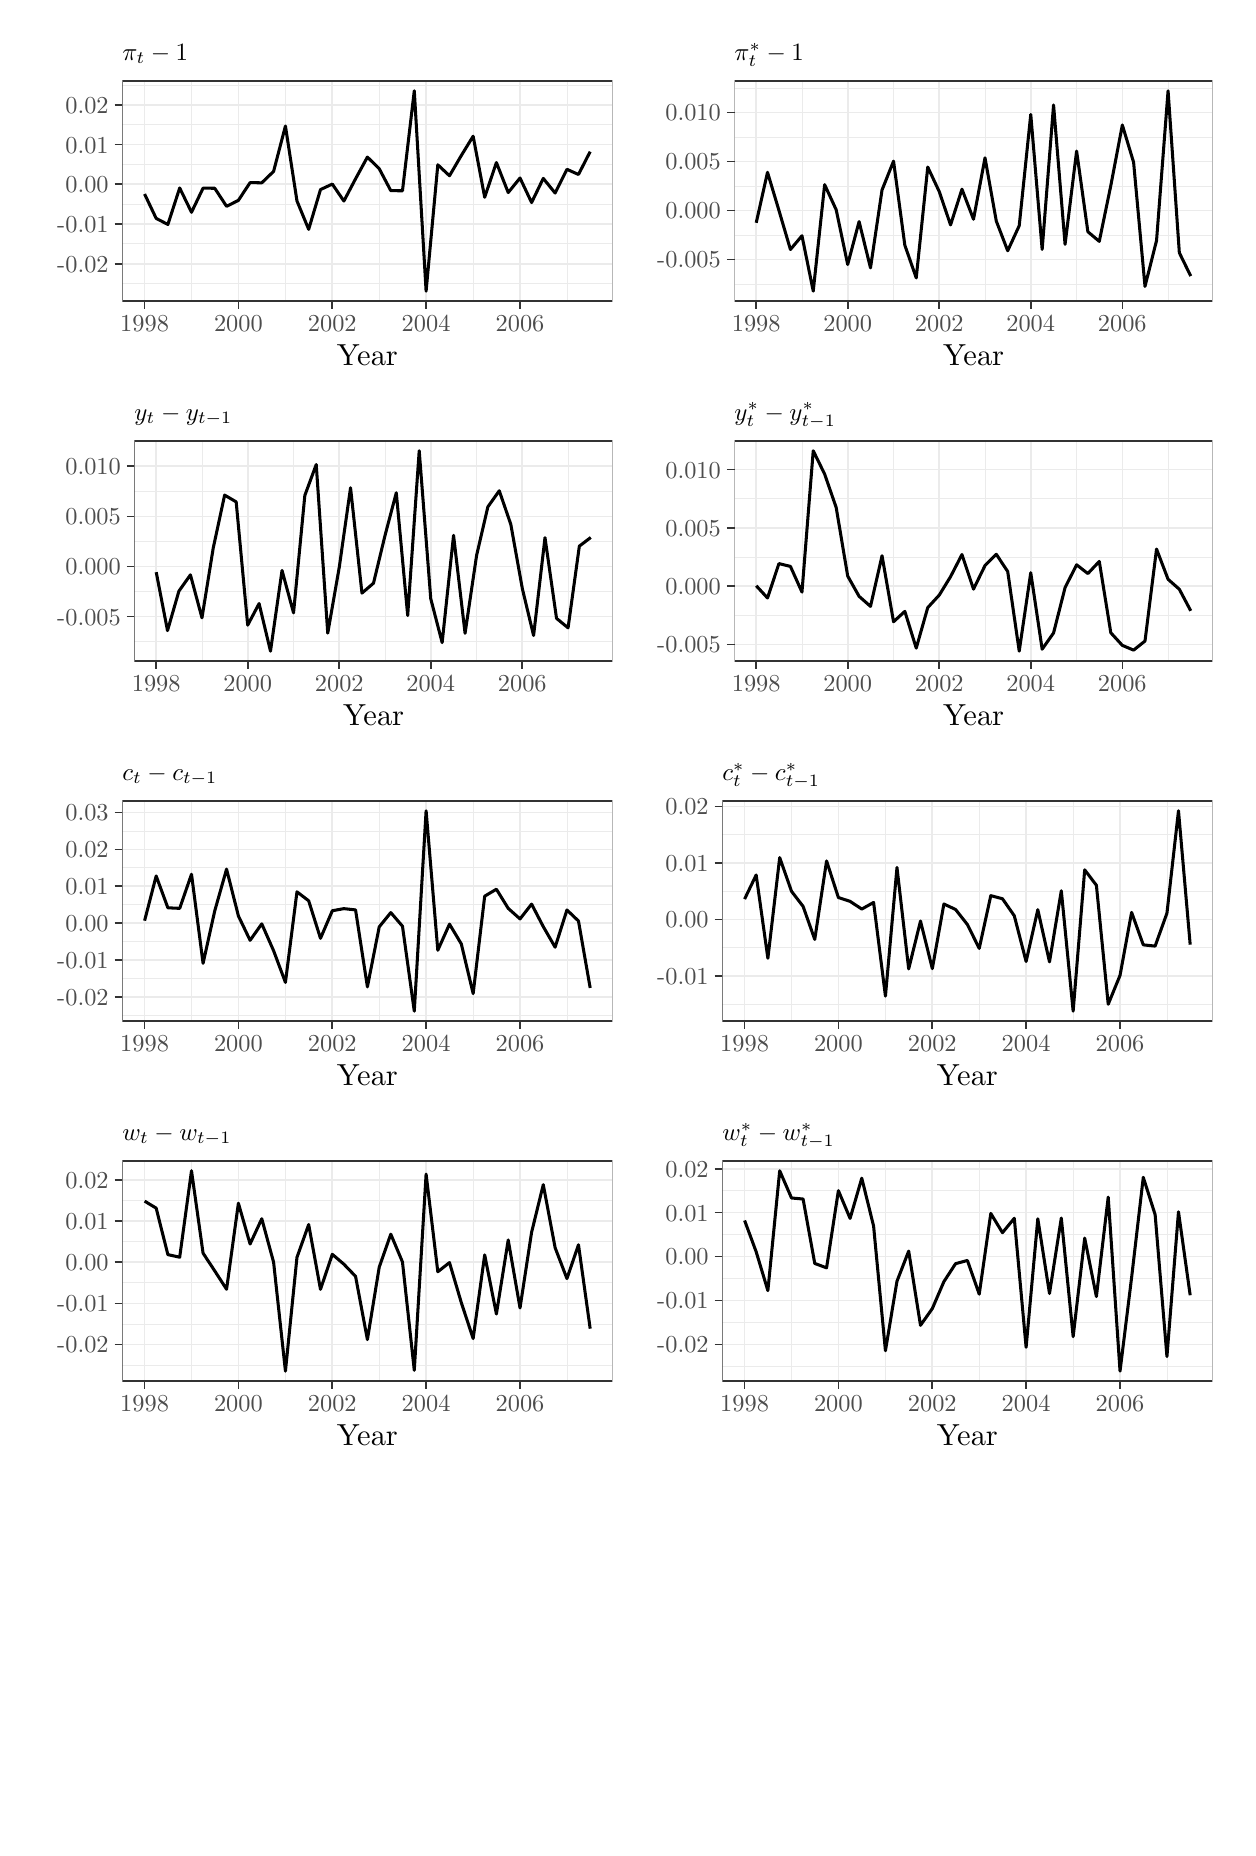
\begin{tikzpicture}[x=1pt,y=1pt]
\definecolor{fillColor}{RGB}{255,255,255}
\path[use as bounding box,fill=fillColor,fill opacity=0.00] (0,0) rectangle (433.62,650.43);
\begin{scope}
\path[clip] (  0.00,520.34) rectangle (216.81,650.43);
\definecolor{drawColor}{RGB}{255,255,255}
\definecolor{fillColor}{RGB}{255,255,255}

\path[draw=drawColor,line width= 0.6pt,line join=round,line cap=round,fill=fillColor] (  0.00,520.34) rectangle (216.81,650.43);
\end{scope}
\begin{scope}
\path[clip] ( 34.20,551.60) rectangle (211.31,631.24);
\definecolor{fillColor}{RGB}{255,255,255}

\path[fill=fillColor] ( 34.20,551.60) rectangle (211.31,631.24);
\definecolor{drawColor}{gray}{0.92}

\path[draw=drawColor,line width= 0.3pt,line join=round] ( 34.20,557.95) --
	(211.31,557.95);

\path[draw=drawColor,line width= 0.3pt,line join=round] ( 34.20,572.30) --
	(211.31,572.30);

\path[draw=drawColor,line width= 0.3pt,line join=round] ( 34.20,586.65) --
	(211.31,586.65);

\path[draw=drawColor,line width= 0.3pt,line join=round] ( 34.20,601.00) --
	(211.31,601.00);

\path[draw=drawColor,line width= 0.3pt,line join=round] ( 34.20,615.34) --
	(211.31,615.34);

\path[draw=drawColor,line width= 0.3pt,line join=round] ( 34.20,629.69) --
	(211.31,629.69);

\path[draw=drawColor,line width= 0.3pt,line join=round] ( 59.20,551.60) --
	( 59.20,631.24);

\path[draw=drawColor,line width= 0.3pt,line join=round] ( 93.11,551.60) --
	( 93.11,631.24);

\path[draw=drawColor,line width= 0.3pt,line join=round] (127.03,551.60) --
	(127.03,631.24);

\path[draw=drawColor,line width= 0.3pt,line join=round] (160.94,551.60) --
	(160.94,631.24);

\path[draw=drawColor,line width= 0.3pt,line join=round] (194.86,551.60) --
	(194.86,631.24);

\path[draw=drawColor,line width= 0.6pt,line join=round] ( 34.20,565.12) --
	(211.31,565.12);

\path[draw=drawColor,line width= 0.6pt,line join=round] ( 34.20,579.47) --
	(211.31,579.47);

\path[draw=drawColor,line width= 0.6pt,line join=round] ( 34.20,593.82) --
	(211.31,593.82);

\path[draw=drawColor,line width= 0.6pt,line join=round] ( 34.20,608.17) --
	(211.31,608.17);

\path[draw=drawColor,line width= 0.6pt,line join=round] ( 34.20,622.52) --
	(211.31,622.52);

\path[draw=drawColor,line width= 0.6pt,line join=round] ( 42.25,551.60) --
	( 42.25,631.24);

\path[draw=drawColor,line width= 0.6pt,line join=round] ( 76.14,551.60) --
	( 76.14,631.24);

\path[draw=drawColor,line width= 0.6pt,line join=round] (110.08,551.60) --
	(110.08,631.24);

\path[draw=drawColor,line width= 0.6pt,line join=round] (143.97,551.60) --
	(143.97,631.24);

\path[draw=drawColor,line width= 0.6pt,line join=round] (177.91,551.60) --
	(177.91,631.24);
\definecolor{drawColor}{RGB}{0,0,0}

\path[draw=drawColor,line width= 1.1pt,line join=round] ( 42.25,590.30) --
	( 46.43,581.51) --
	( 50.66,579.31) --
	( 54.93,592.50) --
	( 59.20,583.71) --
	( 63.38,592.44) --
	( 67.60,592.39) --
	( 71.87,585.87) --
	( 76.14,588.02) --
	( 80.37,594.44) --
	( 84.59,594.36) --
	( 88.86,598.49) --
	( 93.14,614.88) --
	( 97.31,587.81) --
	(101.54,577.54) --
	(105.81,591.92) --
	(110.08,593.90) --
	(114.26,587.77) --
	(118.48,595.81) --
	(122.76,603.66) --
	(127.03,599.47) --
	(131.21,591.53) --
	(135.43,591.48) --
	(139.70,627.62) --
	(143.97,555.22) --
	(148.20,600.87) --
	(152.42,596.91) --
	(156.69,604.22) --
	(160.97,611.21) --
	(165.14,589.14) --
	(169.37,601.69) --
	(173.64,590.84) --
	(177.91,596.10) --
	(182.09,587.23) --
	(186.31,595.96) --
	(190.59,590.66) --
	(194.86,599.24) --
	(199.03,597.37) --
	(203.26,605.64);
\definecolor{drawColor}{gray}{0.20}

\path[draw=drawColor,line width= 0.6pt,line join=round,line cap=round] ( 34.20,551.60) rectangle (211.31,631.24);
\end{scope}
\begin{scope}
\path[clip] (  0.00,  0.00) rectangle (433.62,650.43);
\definecolor{drawColor}{gray}{0.30}

\node[text=drawColor,anchor=base east,inner sep=0pt, outer sep=0pt, scale=  0.88] at ( 29.25,562.09) {-0.02};

\node[text=drawColor,anchor=base east,inner sep=0pt, outer sep=0pt, scale=  0.88] at ( 29.25,576.44) {-0.01};

\node[text=drawColor,anchor=base east,inner sep=0pt, outer sep=0pt, scale=  0.88] at ( 29.25,590.79) {0.00};

\node[text=drawColor,anchor=base east,inner sep=0pt, outer sep=0pt, scale=  0.88] at ( 29.25,605.14) {0.01};

\node[text=drawColor,anchor=base east,inner sep=0pt, outer sep=0pt, scale=  0.88] at ( 29.25,619.49) {0.02};
\end{scope}
\begin{scope}
\path[clip] (  0.00,  0.00) rectangle (433.62,650.43);
\definecolor{drawColor}{gray}{0.20}

\path[draw=drawColor,line width= 0.6pt,line join=round] ( 31.45,565.12) --
	( 34.20,565.12);

\path[draw=drawColor,line width= 0.6pt,line join=round] ( 31.45,579.47) --
	( 34.20,579.47);

\path[draw=drawColor,line width= 0.6pt,line join=round] ( 31.45,593.82) --
	( 34.20,593.82);

\path[draw=drawColor,line width= 0.6pt,line join=round] ( 31.45,608.17) --
	( 34.20,608.17);

\path[draw=drawColor,line width= 0.6pt,line join=round] ( 31.45,622.52) --
	( 34.20,622.52);
\end{scope}
\begin{scope}
\path[clip] (  0.00,  0.00) rectangle (433.62,650.43);
\definecolor{drawColor}{gray}{0.20}

\path[draw=drawColor,line width= 0.6pt,line join=round] ( 42.25,548.85) --
	( 42.25,551.60);

\path[draw=drawColor,line width= 0.6pt,line join=round] ( 76.14,548.85) --
	( 76.14,551.60);

\path[draw=drawColor,line width= 0.6pt,line join=round] (110.08,548.85) --
	(110.08,551.60);

\path[draw=drawColor,line width= 0.6pt,line join=round] (143.97,548.85) --
	(143.97,551.60);

\path[draw=drawColor,line width= 0.6pt,line join=round] (177.91,548.85) --
	(177.91,551.60);
\end{scope}
\begin{scope}
\path[clip] (  0.00,  0.00) rectangle (433.62,650.43);
\definecolor{drawColor}{gray}{0.30}

\node[text=drawColor,anchor=base,inner sep=0pt, outer sep=0pt, scale=  0.88] at ( 42.25,540.59) {1998};

\node[text=drawColor,anchor=base,inner sep=0pt, outer sep=0pt, scale=  0.88] at ( 76.14,540.59) {2000};

\node[text=drawColor,anchor=base,inner sep=0pt, outer sep=0pt, scale=  0.88] at (110.08,540.59) {2002};

\node[text=drawColor,anchor=base,inner sep=0pt, outer sep=0pt, scale=  0.88] at (143.97,540.59) {2004};

\node[text=drawColor,anchor=base,inner sep=0pt, outer sep=0pt, scale=  0.88] at (177.91,540.59) {2006};
\end{scope}
\begin{scope}
\path[clip] (  0.00,  0.00) rectangle (433.62,650.43);
\definecolor{drawColor}{RGB}{0,0,0}

\node[text=drawColor,anchor=base,inner sep=0pt, outer sep=0pt, scale=  1.10] at (122.76,528.27) {Year};
\end{scope}
\begin{scope}
\path[clip] (  0.00,  0.00) rectangle (433.62,650.43);
\definecolor{drawColor}{RGB}{0,0,0}

\node[text=drawColor,anchor=base west,inner sep=0pt, outer sep=0pt, scale=  0.90] at ( 34.20,638.73) {$\pi_t - 1$};
\end{scope}
\begin{scope}
\path[clip] (216.81,520.34) rectangle (433.62,650.43);
\definecolor{drawColor}{RGB}{255,255,255}
\definecolor{fillColor}{RGB}{255,255,255}

\path[draw=drawColor,line width= 0.6pt,line join=round,line cap=round,fill=fillColor] (216.81,520.34) rectangle (433.62,650.43);
\end{scope}
\begin{scope}
\path[clip] (255.41,551.60) rectangle (428.12,631.24);
\definecolor{fillColor}{RGB}{255,255,255}

\path[fill=fillColor] (255.41,551.60) rectangle (428.12,631.24);
\definecolor{drawColor}{gray}{0.92}

\path[draw=drawColor,line width= 0.3pt,line join=round] (255.41,557.81) --
	(428.12,557.81);

\path[draw=drawColor,line width= 0.3pt,line join=round] (255.41,575.51) --
	(428.12,575.51);

\path[draw=drawColor,line width= 0.3pt,line join=round] (255.41,593.22) --
	(428.12,593.22);

\path[draw=drawColor,line width= 0.3pt,line join=round] (255.41,610.92) --
	(428.12,610.92);

\path[draw=drawColor,line width= 0.3pt,line join=round] (255.41,628.63) --
	(428.12,628.63);

\path[draw=drawColor,line width= 0.3pt,line join=round] (279.79,551.60) --
	(279.79,631.24);

\path[draw=drawColor,line width= 0.3pt,line join=round] (312.86,551.60) --
	(312.86,631.24);

\path[draw=drawColor,line width= 0.3pt,line join=round] (345.93,551.60) --
	(345.93,631.24);

\path[draw=drawColor,line width= 0.3pt,line join=round] (379.00,551.60) --
	(379.00,631.24);

\path[draw=drawColor,line width= 0.3pt,line join=round] (412.08,551.60) --
	(412.08,631.24);

\path[draw=drawColor,line width= 0.6pt,line join=round] (255.41,566.66) --
	(428.12,566.66);

\path[draw=drawColor,line width= 0.6pt,line join=round] (255.41,584.36) --
	(428.12,584.36);

\path[draw=drawColor,line width= 0.6pt,line join=round] (255.41,602.07) --
	(428.12,602.07);

\path[draw=drawColor,line width= 0.6pt,line join=round] (255.41,619.77) --
	(428.12,619.77);

\path[draw=drawColor,line width= 0.6pt,line join=round] (263.26,551.60) --
	(263.26,631.24);

\path[draw=drawColor,line width= 0.6pt,line join=round] (296.31,551.60) --
	(296.31,631.24);

\path[draw=drawColor,line width= 0.6pt,line join=round] (329.41,551.60) --
	(329.41,631.24);

\path[draw=drawColor,line width= 0.6pt,line join=round] (362.46,551.60) --
	(362.46,631.24);

\path[draw=drawColor,line width= 0.6pt,line join=round] (395.55,551.60) --
	(395.55,631.24);
\definecolor{drawColor}{RGB}{0,0,0}

\path[draw=drawColor,line width= 1.1pt,line join=round] (263.26,579.92) --
	(267.34,598.16) --
	(271.46,584.41) --
	(275.62,570.27) --
	(279.79,575.23) --
	(283.86,555.22) --
	(287.98,593.70) --
	(292.15,584.63) --
	(296.31,564.84) --
	(300.43,580.36) --
	(304.55,563.62) --
	(308.72,591.78) --
	(312.88,602.20) --
	(316.96,571.81) --
	(321.08,560.01) --
	(325.24,600.05) --
	(329.41,591.15) --
	(333.48,579.14) --
	(337.60,592.06) --
	(341.77,581.19) --
	(345.93,603.39) --
	(350.01,580.53) --
	(354.13,569.81) --
	(358.29,578.85) --
	(362.46,619.08) --
	(366.58,570.28) --
	(370.70,622.49) --
	(374.86,572.12) --
	(379.03,605.84) --
	(383.10,576.68) --
	(387.22,573.20) --
	(391.39,593.38) --
	(395.55,615.25) --
	(399.62,601.79) --
	(403.74,556.93) --
	(407.91,573.48) --
	(412.08,627.62) --
	(416.15,569.09) --
	(420.27,560.66);
\definecolor{drawColor}{gray}{0.20}

\path[draw=drawColor,line width= 0.6pt,line join=round,line cap=round] (255.41,551.60) rectangle (428.12,631.24);
\end{scope}
\begin{scope}
\path[clip] (  0.00,  0.00) rectangle (433.62,650.43);
\definecolor{drawColor}{gray}{0.30}

\node[text=drawColor,anchor=base east,inner sep=0pt, outer sep=0pt, scale=  0.88] at (250.46,563.63) {-0.005};

\node[text=drawColor,anchor=base east,inner sep=0pt, outer sep=0pt, scale=  0.88] at (250.46,581.33) {0.000};

\node[text=drawColor,anchor=base east,inner sep=0pt, outer sep=0pt, scale=  0.88] at (250.46,599.04) {0.005};

\node[text=drawColor,anchor=base east,inner sep=0pt, outer sep=0pt, scale=  0.88] at (250.46,616.74) {0.010};
\end{scope}
\begin{scope}
\path[clip] (  0.00,  0.00) rectangle (433.62,650.43);
\definecolor{drawColor}{gray}{0.20}

\path[draw=drawColor,line width= 0.6pt,line join=round] (252.66,566.66) --
	(255.41,566.66);

\path[draw=drawColor,line width= 0.6pt,line join=round] (252.66,584.36) --
	(255.41,584.36);

\path[draw=drawColor,line width= 0.6pt,line join=round] (252.66,602.07) --
	(255.41,602.07);

\path[draw=drawColor,line width= 0.6pt,line join=round] (252.66,619.77) --
	(255.41,619.77);
\end{scope}
\begin{scope}
\path[clip] (  0.00,  0.00) rectangle (433.62,650.43);
\definecolor{drawColor}{gray}{0.20}

\path[draw=drawColor,line width= 0.6pt,line join=round] (263.26,548.85) --
	(263.26,551.60);

\path[draw=drawColor,line width= 0.6pt,line join=round] (296.31,548.85) --
	(296.31,551.60);

\path[draw=drawColor,line width= 0.6pt,line join=round] (329.41,548.85) --
	(329.41,551.60);

\path[draw=drawColor,line width= 0.6pt,line join=round] (362.46,548.85) --
	(362.46,551.60);

\path[draw=drawColor,line width= 0.6pt,line join=round] (395.55,548.85) --
	(395.55,551.60);
\end{scope}
\begin{scope}
\path[clip] (  0.00,  0.00) rectangle (433.62,650.43);
\definecolor{drawColor}{gray}{0.30}

\node[text=drawColor,anchor=base,inner sep=0pt, outer sep=0pt, scale=  0.88] at (263.26,540.59) {1998};

\node[text=drawColor,anchor=base,inner sep=0pt, outer sep=0pt, scale=  0.88] at (296.31,540.59) {2000};

\node[text=drawColor,anchor=base,inner sep=0pt, outer sep=0pt, scale=  0.88] at (329.41,540.59) {2002};

\node[text=drawColor,anchor=base,inner sep=0pt, outer sep=0pt, scale=  0.88] at (362.46,540.59) {2004};

\node[text=drawColor,anchor=base,inner sep=0pt, outer sep=0pt, scale=  0.88] at (395.55,540.59) {2006};
\end{scope}
\begin{scope}
\path[clip] (  0.00,  0.00) rectangle (433.62,650.43);
\definecolor{drawColor}{RGB}{0,0,0}

\node[text=drawColor,anchor=base,inner sep=0pt, outer sep=0pt, scale=  1.10] at (341.77,528.27) {Year};
\end{scope}
\begin{scope}
\path[clip] (  0.00,  0.00) rectangle (433.62,650.43);
\definecolor{drawColor}{RGB}{0,0,0}

\node[text=drawColor,anchor=base west,inner sep=0pt, outer sep=0pt, scale=  0.90] at (255.41,638.73) {$\pi^{*}_t - 1$};
\end{scope}
\begin{scope}
\path[clip] (  0.00,390.26) rectangle (216.81,520.34);
\definecolor{drawColor}{RGB}{255,255,255}
\definecolor{fillColor}{RGB}{255,255,255}

\path[draw=drawColor,line width= 0.6pt,line join=round,line cap=round,fill=fillColor] ( -0.00,390.26) rectangle (216.81,520.34);
\end{scope}
\begin{scope}
\path[clip] ( 38.60,421.51) rectangle (211.31,501.16);
\definecolor{fillColor}{RGB}{255,255,255}

\path[fill=fillColor] ( 38.60,421.51) rectangle (211.31,501.16);
\definecolor{drawColor}{gray}{0.92}

\path[draw=drawColor,line width= 0.3pt,line join=round] ( 38.60,428.56) --
	(211.31,428.56);

\path[draw=drawColor,line width= 0.3pt,line join=round] ( 38.60,446.67) --
	(211.31,446.67);

\path[draw=drawColor,line width= 0.3pt,line join=round] ( 38.60,464.79) --
	(211.31,464.79);

\path[draw=drawColor,line width= 0.3pt,line join=round] ( 38.60,482.90) --
	(211.31,482.90);

\path[draw=drawColor,line width= 0.3pt,line join=round] ( 38.60,501.01) --
	(211.31,501.01);

\path[draw=drawColor,line width= 0.3pt,line join=round] ( 62.98,421.51) --
	( 62.98,501.16);

\path[draw=drawColor,line width= 0.3pt,line join=round] ( 96.05,421.51) --
	( 96.05,501.16);

\path[draw=drawColor,line width= 0.3pt,line join=round] (129.12,421.51) --
	(129.12,501.16);

\path[draw=drawColor,line width= 0.3pt,line join=round] (162.19,421.51) --
	(162.19,501.16);

\path[draw=drawColor,line width= 0.3pt,line join=round] (195.27,421.51) --
	(195.27,501.16);

\path[draw=drawColor,line width= 0.6pt,line join=round] ( 38.60,437.61) --
	(211.31,437.61);

\path[draw=drawColor,line width= 0.6pt,line join=round] ( 38.60,455.73) --
	(211.31,455.73);

\path[draw=drawColor,line width= 0.6pt,line join=round] ( 38.60,473.84) --
	(211.31,473.84);

\path[draw=drawColor,line width= 0.6pt,line join=round] ( 38.60,491.96) --
	(211.31,491.96);

\path[draw=drawColor,line width= 0.6pt,line join=round] ( 46.45,421.51) --
	( 46.45,501.16);

\path[draw=drawColor,line width= 0.6pt,line join=round] ( 79.50,421.51) --
	( 79.50,501.16);

\path[draw=drawColor,line width= 0.6pt,line join=round] (112.60,421.51) --
	(112.60,501.16);

\path[draw=drawColor,line width= 0.6pt,line join=round] (145.65,421.51) --
	(145.65,501.16);

\path[draw=drawColor,line width= 0.6pt,line join=round] (178.74,421.51) --
	(178.74,501.16);
\definecolor{drawColor}{RGB}{0,0,0}

\path[draw=drawColor,line width= 1.1pt,line join=round] ( 46.45,453.67) --
	( 50.53,432.55) --
	( 54.65,446.83) --
	( 58.81,452.70) --
	( 62.98,437.16) --
	( 67.05,462.39) --
	( 71.17,481.52) --
	( 75.34,479.07) --
	( 79.50,434.52) --
	( 83.62,442.32) --
	( 87.74,425.13) --
	( 91.91,454.30) --
	( 96.07,438.97) --
	(100.15,481.39) --
	(104.27,492.57) --
	(108.43,431.64) --
	(112.60,455.51) --
	(116.67,484.17) --
	(120.79,446.11) --
	(124.96,449.68) --
	(129.12,466.92) --
	(133.20,482.37) --
	(137.32,438.01) --
	(141.48,497.54) --
	(145.65,444.08) --
	(149.77,428.21) --
	(153.89,466.98) --
	(158.05,431.58) --
	(162.22,459.75) --
	(166.29,477.28) --
	(170.41,483.08) --
	(174.58,470.94) --
	(178.74,447.75) --
	(182.81,430.78) --
	(186.93,466.14) --
	(191.10,436.98) --
	(195.27,433.55) --
	(199.34,463.07) --
	(203.46,466.21);
\definecolor{drawColor}{gray}{0.20}

\path[draw=drawColor,line width= 0.6pt,line join=round,line cap=round] ( 38.60,421.51) rectangle (211.31,501.16);
\end{scope}
\begin{scope}
\path[clip] (  0.00,  0.00) rectangle (433.62,650.43);
\definecolor{drawColor}{gray}{0.30}

\node[text=drawColor,anchor=base east,inner sep=0pt, outer sep=0pt, scale=  0.88] at ( 33.65,434.58) {-0.005};

\node[text=drawColor,anchor=base east,inner sep=0pt, outer sep=0pt, scale=  0.88] at ( 33.65,452.70) {0.000};

\node[text=drawColor,anchor=base east,inner sep=0pt, outer sep=0pt, scale=  0.88] at ( 33.65,470.81) {0.005};

\node[text=drawColor,anchor=base east,inner sep=0pt, outer sep=0pt, scale=  0.88] at ( 33.65,488.93) {0.010};
\end{scope}
\begin{scope}
\path[clip] (  0.00,  0.00) rectangle (433.62,650.43);
\definecolor{drawColor}{gray}{0.20}

\path[draw=drawColor,line width= 0.6pt,line join=round] ( 35.85,437.61) --
	( 38.60,437.61);

\path[draw=drawColor,line width= 0.6pt,line join=round] ( 35.85,455.73) --
	( 38.60,455.73);

\path[draw=drawColor,line width= 0.6pt,line join=round] ( 35.85,473.84) --
	( 38.60,473.84);

\path[draw=drawColor,line width= 0.6pt,line join=round] ( 35.85,491.96) --
	( 38.60,491.96);
\end{scope}
\begin{scope}
\path[clip] (  0.00,  0.00) rectangle (433.62,650.43);
\definecolor{drawColor}{gray}{0.20}

\path[draw=drawColor,line width= 0.6pt,line join=round] ( 46.45,418.76) --
	( 46.45,421.51);

\path[draw=drawColor,line width= 0.6pt,line join=round] ( 79.50,418.76) --
	( 79.50,421.51);

\path[draw=drawColor,line width= 0.6pt,line join=round] (112.60,418.76) --
	(112.60,421.51);

\path[draw=drawColor,line width= 0.6pt,line join=round] (145.65,418.76) --
	(145.65,421.51);

\path[draw=drawColor,line width= 0.6pt,line join=round] (178.74,418.76) --
	(178.74,421.51);
\end{scope}
\begin{scope}
\path[clip] (  0.00,  0.00) rectangle (433.62,650.43);
\definecolor{drawColor}{gray}{0.30}

\node[text=drawColor,anchor=base,inner sep=0pt, outer sep=0pt, scale=  0.88] at ( 46.45,410.50) {1998};

\node[text=drawColor,anchor=base,inner sep=0pt, outer sep=0pt, scale=  0.88] at ( 79.50,410.50) {2000};

\node[text=drawColor,anchor=base,inner sep=0pt, outer sep=0pt, scale=  0.88] at (112.60,410.50) {2002};

\node[text=drawColor,anchor=base,inner sep=0pt, outer sep=0pt, scale=  0.88] at (145.65,410.50) {2004};

\node[text=drawColor,anchor=base,inner sep=0pt, outer sep=0pt, scale=  0.88] at (178.74,410.50) {2006};
\end{scope}
\begin{scope}
\path[clip] (  0.00,  0.00) rectangle (433.62,650.43);
\definecolor{drawColor}{RGB}{0,0,0}

\node[text=drawColor,anchor=base,inner sep=0pt, outer sep=0pt, scale=  1.10] at (124.96,398.19) {Year};
\end{scope}
\begin{scope}
\path[clip] (  0.00,  0.00) rectangle (433.62,650.43);
\definecolor{drawColor}{RGB}{0,0,0}

\node[text=drawColor,anchor=base west,inner sep=0pt, outer sep=0pt, scale=  0.90] at ( 38.60,508.65) {$y_t - y_{t-1}$};
\end{scope}
\begin{scope}
\path[clip] (216.81,390.26) rectangle (433.62,520.34);
\definecolor{drawColor}{RGB}{255,255,255}
\definecolor{fillColor}{RGB}{255,255,255}

\path[draw=drawColor,line width= 0.6pt,line join=round,line cap=round,fill=fillColor] (216.81,390.26) rectangle (433.62,520.34);
\end{scope}
\begin{scope}
\path[clip] (255.41,421.51) rectangle (428.12,501.16);
\definecolor{fillColor}{RGB}{255,255,255}

\path[fill=fillColor] (255.41,421.51) rectangle (428.12,501.16);
\definecolor{drawColor}{gray}{0.92}

\path[draw=drawColor,line width= 0.3pt,line join=round] (255.41,438.10) --
	(428.12,438.10);

\path[draw=drawColor,line width= 0.3pt,line join=round] (255.41,459.15) --
	(428.12,459.15);

\path[draw=drawColor,line width= 0.3pt,line join=round] (255.41,480.19) --
	(428.12,480.19);

\path[draw=drawColor,line width= 0.3pt,line join=round] (279.79,421.51) --
	(279.79,501.16);

\path[draw=drawColor,line width= 0.3pt,line join=round] (312.86,421.51) --
	(312.86,501.16);

\path[draw=drawColor,line width= 0.3pt,line join=round] (345.93,421.51) --
	(345.93,501.16);

\path[draw=drawColor,line width= 0.3pt,line join=round] (379.00,421.51) --
	(379.00,501.16);

\path[draw=drawColor,line width= 0.3pt,line join=round] (412.08,421.51) --
	(412.08,501.16);

\path[draw=drawColor,line width= 0.6pt,line join=round] (255.41,427.58) --
	(428.12,427.58);

\path[draw=drawColor,line width= 0.6pt,line join=round] (255.41,448.62) --
	(428.12,448.62);

\path[draw=drawColor,line width= 0.6pt,line join=round] (255.41,469.67) --
	(428.12,469.67);

\path[draw=drawColor,line width= 0.6pt,line join=round] (255.41,490.71) --
	(428.12,490.71);

\path[draw=drawColor,line width= 0.6pt,line join=round] (263.26,421.51) --
	(263.26,501.16);

\path[draw=drawColor,line width= 0.6pt,line join=round] (296.31,421.51) --
	(296.31,501.16);

\path[draw=drawColor,line width= 0.6pt,line join=round] (329.41,421.51) --
	(329.41,501.16);

\path[draw=drawColor,line width= 0.6pt,line join=round] (362.46,421.51) --
	(362.46,501.16);

\path[draw=drawColor,line width= 0.6pt,line join=round] (395.55,421.51) --
	(395.55,501.16);
\definecolor{drawColor}{RGB}{0,0,0}

\path[draw=drawColor,line width= 1.1pt,line join=round] (263.26,448.76) --
	(267.34,444.34) --
	(271.46,456.77) --
	(275.62,455.75) --
	(279.79,446.47) --
	(283.86,497.54) --
	(287.98,489.11) --
	(292.15,477.05) --
	(296.31,452.27) --
	(300.43,444.94) --
	(304.55,441.31) --
	(308.72,459.61) --
	(312.88,435.75) --
	(316.96,439.51) --
	(321.08,426.22) --
	(325.24,440.87) --
	(329.41,445.41) --
	(333.48,452.05) --
	(337.60,460.05) --
	(341.77,447.54) --
	(345.93,456.06) --
	(350.01,460.13) --
	(354.13,453.91) --
	(358.29,425.13) --
	(362.46,453.47) --
	(366.58,425.83) --
	(370.70,431.71) --
	(374.86,448.09) --
	(379.03,456.34) --
	(383.10,453.16) --
	(387.22,457.56) --
	(391.39,431.76) --
	(395.55,427.22) --
	(399.62,425.50) --
	(403.74,428.79) --
	(407.91,462.03) --
	(412.08,451.10) --
	(416.15,447.49) --
	(420.27,439.71);
\definecolor{drawColor}{gray}{0.20}

\path[draw=drawColor,line width= 0.6pt,line join=round,line cap=round] (255.41,421.51) rectangle (428.12,501.16);
\end{scope}
\begin{scope}
\path[clip] (  0.00,  0.00) rectangle (433.62,650.43);
\definecolor{drawColor}{gray}{0.30}

\node[text=drawColor,anchor=base east,inner sep=0pt, outer sep=0pt, scale=  0.88] at (250.46,424.55) {-0.005};

\node[text=drawColor,anchor=base east,inner sep=0pt, outer sep=0pt, scale=  0.88] at (250.46,445.59) {0.000};

\node[text=drawColor,anchor=base east,inner sep=0pt, outer sep=0pt, scale=  0.88] at (250.46,466.64) {0.005};

\node[text=drawColor,anchor=base east,inner sep=0pt, outer sep=0pt, scale=  0.88] at (250.46,487.68) {0.010};
\end{scope}
\begin{scope}
\path[clip] (  0.00,  0.00) rectangle (433.62,650.43);
\definecolor{drawColor}{gray}{0.20}

\path[draw=drawColor,line width= 0.6pt,line join=round] (252.66,427.58) --
	(255.41,427.58);

\path[draw=drawColor,line width= 0.6pt,line join=round] (252.66,448.62) --
	(255.41,448.62);

\path[draw=drawColor,line width= 0.6pt,line join=round] (252.66,469.67) --
	(255.41,469.67);

\path[draw=drawColor,line width= 0.6pt,line join=round] (252.66,490.71) --
	(255.41,490.71);
\end{scope}
\begin{scope}
\path[clip] (  0.00,  0.00) rectangle (433.62,650.43);
\definecolor{drawColor}{gray}{0.20}

\path[draw=drawColor,line width= 0.6pt,line join=round] (263.26,418.76) --
	(263.26,421.51);

\path[draw=drawColor,line width= 0.6pt,line join=round] (296.31,418.76) --
	(296.31,421.51);

\path[draw=drawColor,line width= 0.6pt,line join=round] (329.41,418.76) --
	(329.41,421.51);

\path[draw=drawColor,line width= 0.6pt,line join=round] (362.46,418.76) --
	(362.46,421.51);

\path[draw=drawColor,line width= 0.6pt,line join=round] (395.55,418.76) --
	(395.55,421.51);
\end{scope}
\begin{scope}
\path[clip] (  0.00,  0.00) rectangle (433.62,650.43);
\definecolor{drawColor}{gray}{0.30}

\node[text=drawColor,anchor=base,inner sep=0pt, outer sep=0pt, scale=  0.88] at (263.26,410.50) {1998};

\node[text=drawColor,anchor=base,inner sep=0pt, outer sep=0pt, scale=  0.88] at (296.31,410.50) {2000};

\node[text=drawColor,anchor=base,inner sep=0pt, outer sep=0pt, scale=  0.88] at (329.41,410.50) {2002};

\node[text=drawColor,anchor=base,inner sep=0pt, outer sep=0pt, scale=  0.88] at (362.46,410.50) {2004};

\node[text=drawColor,anchor=base,inner sep=0pt, outer sep=0pt, scale=  0.88] at (395.55,410.50) {2006};
\end{scope}
\begin{scope}
\path[clip] (  0.00,  0.00) rectangle (433.62,650.43);
\definecolor{drawColor}{RGB}{0,0,0}

\node[text=drawColor,anchor=base,inner sep=0pt, outer sep=0pt, scale=  1.10] at (341.77,398.19) {Year};
\end{scope}
\begin{scope}
\path[clip] (  0.00,  0.00) rectangle (433.62,650.43);
\definecolor{drawColor}{RGB}{0,0,0}

\node[text=drawColor,anchor=base west,inner sep=0pt, outer sep=0pt, scale=  0.90] at (255.41,508.65) {$y^*_t - y^*_{t-1}$};
\end{scope}
\begin{scope}
\path[clip] (  0.00,260.17) rectangle (216.81,390.26);
\definecolor{drawColor}{RGB}{255,255,255}
\definecolor{fillColor}{RGB}{255,255,255}

\path[draw=drawColor,line width= 0.6pt,line join=round,line cap=round,fill=fillColor] (  0.00,260.17) rectangle (216.81,390.26);
\end{scope}
\begin{scope}
\path[clip] ( 34.20,291.43) rectangle (211.31,371.07);
\definecolor{fillColor}{RGB}{255,255,255}

\path[fill=fillColor] ( 34.20,291.43) rectangle (211.31,371.07);
\definecolor{drawColor}{gray}{0.92}

\path[draw=drawColor,line width= 0.3pt,line join=round] ( 34.20,293.60) --
	(211.31,293.60);

\path[draw=drawColor,line width= 0.3pt,line join=round] ( 34.20,306.91) --
	(211.31,306.91);

\path[draw=drawColor,line width= 0.3pt,line join=round] ( 34.20,320.22) --
	(211.31,320.22);

\path[draw=drawColor,line width= 0.3pt,line join=round] ( 34.20,333.53) --
	(211.31,333.53);

\path[draw=drawColor,line width= 0.3pt,line join=round] ( 34.20,346.84) --
	(211.31,346.84);

\path[draw=drawColor,line width= 0.3pt,line join=round] ( 34.20,360.15) --
	(211.31,360.15);

\path[draw=drawColor,line width= 0.3pt,line join=round] ( 59.20,291.43) --
	( 59.20,371.07);

\path[draw=drawColor,line width= 0.3pt,line join=round] ( 93.11,291.43) --
	( 93.11,371.07);

\path[draw=drawColor,line width= 0.3pt,line join=round] (127.03,291.43) --
	(127.03,371.07);

\path[draw=drawColor,line width= 0.3pt,line join=round] (160.94,291.43) --
	(160.94,371.07);

\path[draw=drawColor,line width= 0.3pt,line join=round] (194.86,291.43) --
	(194.86,371.07);

\path[draw=drawColor,line width= 0.6pt,line join=round] ( 34.20,300.25) --
	(211.31,300.25);

\path[draw=drawColor,line width= 0.6pt,line join=round] ( 34.20,313.56) --
	(211.31,313.56);

\path[draw=drawColor,line width= 0.6pt,line join=round] ( 34.20,326.87) --
	(211.31,326.87);

\path[draw=drawColor,line width= 0.6pt,line join=round] ( 34.20,340.18) --
	(211.31,340.18);

\path[draw=drawColor,line width= 0.6pt,line join=round] ( 34.20,353.49) --
	(211.31,353.49);

\path[draw=drawColor,line width= 0.6pt,line join=round] ( 34.20,366.81) --
	(211.31,366.81);

\path[draw=drawColor,line width= 0.6pt,line join=round] ( 42.25,291.43) --
	( 42.25,371.07);

\path[draw=drawColor,line width= 0.6pt,line join=round] ( 76.14,291.43) --
	( 76.14,371.07);

\path[draw=drawColor,line width= 0.6pt,line join=round] (110.08,291.43) --
	(110.08,371.07);

\path[draw=drawColor,line width= 0.6pt,line join=round] (143.97,291.43) --
	(143.97,371.07);

\path[draw=drawColor,line width= 0.6pt,line join=round] (177.91,291.43) --
	(177.91,371.07);
\definecolor{drawColor}{RGB}{0,0,0}

\path[draw=drawColor,line width= 1.1pt,line join=round] ( 42.25,327.73) --
	( 46.43,343.90) --
	( 50.66,332.39) --
	( 54.93,332.19) --
	( 59.20,344.53) --
	( 63.38,312.32) --
	( 67.60,331.29) --
	( 71.87,346.36) --
	( 76.14,329.47) --
	( 80.37,320.64) --
	( 84.59,326.59) --
	( 88.86,316.89) --
	( 93.14,305.43) --
	( 97.31,338.17) --
	(101.54,334.92) --
	(105.81,321.36) --
	(110.08,331.33) --
	(114.26,332.09) --
	(118.48,331.63) --
	(122.76,303.82) --
	(127.03,325.51) --
	(131.21,330.66) --
	(135.43,325.75) --
	(139.70,295.05) --
	(143.97,367.45) --
	(148.20,317.05) --
	(152.42,326.48) --
	(156.69,319.35) --
	(160.97,301.39) --
	(165.14,336.59) --
	(169.37,339.11) --
	(173.64,332.19) --
	(177.91,328.37) --
	(182.09,333.73) --
	(186.31,325.59) --
	(190.59,318.15) --
	(194.86,331.61) --
	(199.03,327.62) --
	(203.26,303.43);
\definecolor{drawColor}{gray}{0.20}

\path[draw=drawColor,line width= 0.6pt,line join=round,line cap=round] ( 34.20,291.43) rectangle (211.31,371.07);
\end{scope}
\begin{scope}
\path[clip] (  0.00,  0.00) rectangle (433.62,650.43);
\definecolor{drawColor}{gray}{0.30}

\node[text=drawColor,anchor=base east,inner sep=0pt, outer sep=0pt, scale=  0.88] at ( 29.25,297.22) {-0.02};

\node[text=drawColor,anchor=base east,inner sep=0pt, outer sep=0pt, scale=  0.88] at ( 29.25,310.53) {-0.01};

\node[text=drawColor,anchor=base east,inner sep=0pt, outer sep=0pt, scale=  0.88] at ( 29.25,323.84) {0.00};

\node[text=drawColor,anchor=base east,inner sep=0pt, outer sep=0pt, scale=  0.88] at ( 29.25,337.15) {0.01};

\node[text=drawColor,anchor=base east,inner sep=0pt, outer sep=0pt, scale=  0.88] at ( 29.25,350.46) {0.02};

\node[text=drawColor,anchor=base east,inner sep=0pt, outer sep=0pt, scale=  0.88] at ( 29.25,363.78) {0.03};
\end{scope}
\begin{scope}
\path[clip] (  0.00,  0.00) rectangle (433.62,650.43);
\definecolor{drawColor}{gray}{0.20}

\path[draw=drawColor,line width= 0.6pt,line join=round] ( 31.45,300.25) --
	( 34.20,300.25);

\path[draw=drawColor,line width= 0.6pt,line join=round] ( 31.45,313.56) --
	( 34.20,313.56);

\path[draw=drawColor,line width= 0.6pt,line join=round] ( 31.45,326.87) --
	( 34.20,326.87);

\path[draw=drawColor,line width= 0.6pt,line join=round] ( 31.45,340.18) --
	( 34.20,340.18);

\path[draw=drawColor,line width= 0.6pt,line join=round] ( 31.45,353.49) --
	( 34.20,353.49);

\path[draw=drawColor,line width= 0.6pt,line join=round] ( 31.45,366.81) --
	( 34.20,366.81);
\end{scope}
\begin{scope}
\path[clip] (  0.00,  0.00) rectangle (433.62,650.43);
\definecolor{drawColor}{gray}{0.20}

\path[draw=drawColor,line width= 0.6pt,line join=round] ( 42.25,288.68) --
	( 42.25,291.43);

\path[draw=drawColor,line width= 0.6pt,line join=round] ( 76.14,288.68) --
	( 76.14,291.43);

\path[draw=drawColor,line width= 0.6pt,line join=round] (110.08,288.68) --
	(110.08,291.43);

\path[draw=drawColor,line width= 0.6pt,line join=round] (143.97,288.68) --
	(143.97,291.43);

\path[draw=drawColor,line width= 0.6pt,line join=round] (177.91,288.68) --
	(177.91,291.43);
\end{scope}
\begin{scope}
\path[clip] (  0.00,  0.00) rectangle (433.62,650.43);
\definecolor{drawColor}{gray}{0.30}

\node[text=drawColor,anchor=base,inner sep=0pt, outer sep=0pt, scale=  0.88] at ( 42.25,280.41) {1998};

\node[text=drawColor,anchor=base,inner sep=0pt, outer sep=0pt, scale=  0.88] at ( 76.14,280.41) {2000};

\node[text=drawColor,anchor=base,inner sep=0pt, outer sep=0pt, scale=  0.88] at (110.08,280.41) {2002};

\node[text=drawColor,anchor=base,inner sep=0pt, outer sep=0pt, scale=  0.88] at (143.97,280.41) {2004};

\node[text=drawColor,anchor=base,inner sep=0pt, outer sep=0pt, scale=  0.88] at (177.91,280.41) {2006};
\end{scope}
\begin{scope}
\path[clip] (  0.00,  0.00) rectangle (433.62,650.43);
\definecolor{drawColor}{RGB}{0,0,0}

\node[text=drawColor,anchor=base,inner sep=0pt, outer sep=0pt, scale=  1.10] at (122.76,268.10) {Year};
\end{scope}
\begin{scope}
\path[clip] (  0.00,  0.00) rectangle (433.62,650.43);
\definecolor{drawColor}{RGB}{0,0,0}

\node[text=drawColor,anchor=base west,inner sep=0pt, outer sep=0pt, scale=  0.90] at ( 34.20,378.56) {$c_t - c_{t-1}$};
\end{scope}
\begin{scope}
\path[clip] (216.81,260.17) rectangle (433.62,390.26);
\definecolor{drawColor}{RGB}{255,255,255}
\definecolor{fillColor}{RGB}{255,255,255}

\path[draw=drawColor,line width= 0.6pt,line join=round,line cap=round,fill=fillColor] (216.81,260.17) rectangle (433.62,390.26);
\end{scope}
\begin{scope}
\path[clip] (251.01,291.43) rectangle (428.12,371.07);
\definecolor{fillColor}{RGB}{255,255,255}

\path[fill=fillColor] (251.01,291.43) rectangle (428.12,371.07);
\definecolor{drawColor}{gray}{0.92}

\path[draw=drawColor,line width= 0.3pt,line join=round] (251.01,297.56) --
	(428.12,297.56);

\path[draw=drawColor,line width= 0.3pt,line join=round] (251.01,317.97) --
	(428.12,317.97);

\path[draw=drawColor,line width= 0.3pt,line join=round] (251.01,338.38) --
	(428.12,338.38);

\path[draw=drawColor,line width= 0.3pt,line join=round] (251.01,358.79) --
	(428.12,358.79);

\path[draw=drawColor,line width= 0.3pt,line join=round] (276.01,291.43) --
	(276.01,371.07);

\path[draw=drawColor,line width= 0.3pt,line join=round] (309.92,291.43) --
	(309.92,371.07);

\path[draw=drawColor,line width= 0.3pt,line join=round] (343.84,291.43) --
	(343.84,371.07);

\path[draw=drawColor,line width= 0.3pt,line join=round] (377.75,291.43) --
	(377.75,371.07);

\path[draw=drawColor,line width= 0.3pt,line join=round] (411.67,291.43) --
	(411.67,371.07);

\path[draw=drawColor,line width= 0.6pt,line join=round] (251.01,307.77) --
	(428.12,307.77);

\path[draw=drawColor,line width= 0.6pt,line join=round] (251.01,328.18) --
	(428.12,328.18);

\path[draw=drawColor,line width= 0.6pt,line join=round] (251.01,348.59) --
	(428.12,348.59);

\path[draw=drawColor,line width= 0.6pt,line join=round] (251.01,369.00) --
	(428.12,369.00);

\path[draw=drawColor,line width= 0.6pt,line join=round] (259.06,291.43) --
	(259.06,371.07);

\path[draw=drawColor,line width= 0.6pt,line join=round] (292.95,291.43) --
	(292.95,371.07);

\path[draw=drawColor,line width= 0.6pt,line join=round] (326.89,291.43) --
	(326.89,371.07);

\path[draw=drawColor,line width= 0.6pt,line join=round] (360.78,291.43) --
	(360.78,371.07);

\path[draw=drawColor,line width= 0.6pt,line join=round] (394.72,291.43) --
	(394.72,371.07);
\definecolor{drawColor}{RGB}{0,0,0}

\path[draw=drawColor,line width= 1.1pt,line join=round] (259.06,335.54) --
	(263.24,344.26) --
	(267.47,314.15) --
	(271.74,350.54) --
	(276.01,338.35) --
	(280.19,332.91) --
	(284.41,320.96) --
	(288.68,349.33) --
	(292.95,336.10) --
	(297.18,334.72) --
	(301.40,331.93) --
	(305.67,334.33) --
	(309.95,300.47) --
	(314.12,346.95) --
	(318.35,310.31) --
	(322.62,327.61) --
	(326.89,310.41) --
	(331.07,333.76) --
	(335.29,331.79) --
	(339.57,326.34) --
	(343.84,317.71) --
	(348.02,336.78) --
	(352.24,335.66) --
	(356.51,329.51) --
	(360.78,312.98) --
	(365.01,331.70) --
	(369.23,312.85) --
	(373.50,338.56) --
	(377.78,295.05) --
	(381.95,346.11) --
	(386.18,340.52) --
	(390.45,297.54) --
	(394.72,307.97) --
	(398.90,330.74) --
	(403.12,319.00) --
	(407.40,318.55) --
	(411.67,330.44) --
	(415.84,367.45) --
	(420.07,319.07);
\definecolor{drawColor}{gray}{0.20}

\path[draw=drawColor,line width= 0.6pt,line join=round,line cap=round] (251.01,291.43) rectangle (428.12,371.07);
\end{scope}
\begin{scope}
\path[clip] (  0.00,  0.00) rectangle (433.62,650.43);
\definecolor{drawColor}{gray}{0.30}

\node[text=drawColor,anchor=base east,inner sep=0pt, outer sep=0pt, scale=  0.88] at (246.06,304.74) {-0.01};

\node[text=drawColor,anchor=base east,inner sep=0pt, outer sep=0pt, scale=  0.88] at (246.06,325.15) {0.00};

\node[text=drawColor,anchor=base east,inner sep=0pt, outer sep=0pt, scale=  0.88] at (246.06,345.56) {0.01};

\node[text=drawColor,anchor=base east,inner sep=0pt, outer sep=0pt, scale=  0.88] at (246.06,365.97) {0.02};
\end{scope}
\begin{scope}
\path[clip] (  0.00,  0.00) rectangle (433.62,650.43);
\definecolor{drawColor}{gray}{0.20}

\path[draw=drawColor,line width= 0.6pt,line join=round] (248.26,307.77) --
	(251.01,307.77);

\path[draw=drawColor,line width= 0.6pt,line join=round] (248.26,328.18) --
	(251.01,328.18);

\path[draw=drawColor,line width= 0.6pt,line join=round] (248.26,348.59) --
	(251.01,348.59);

\path[draw=drawColor,line width= 0.6pt,line join=round] (248.26,369.00) --
	(251.01,369.00);
\end{scope}
\begin{scope}
\path[clip] (  0.00,  0.00) rectangle (433.62,650.43);
\definecolor{drawColor}{gray}{0.20}

\path[draw=drawColor,line width= 0.6pt,line join=round] (259.06,288.68) --
	(259.06,291.43);

\path[draw=drawColor,line width= 0.6pt,line join=round] (292.95,288.68) --
	(292.95,291.43);

\path[draw=drawColor,line width= 0.6pt,line join=round] (326.89,288.68) --
	(326.89,291.43);

\path[draw=drawColor,line width= 0.6pt,line join=round] (360.78,288.68) --
	(360.78,291.43);

\path[draw=drawColor,line width= 0.6pt,line join=round] (394.72,288.68) --
	(394.72,291.43);
\end{scope}
\begin{scope}
\path[clip] (  0.00,  0.00) rectangle (433.62,650.43);
\definecolor{drawColor}{gray}{0.30}

\node[text=drawColor,anchor=base,inner sep=0pt, outer sep=0pt, scale=  0.88] at (259.06,280.41) {1998};

\node[text=drawColor,anchor=base,inner sep=0pt, outer sep=0pt, scale=  0.88] at (292.95,280.41) {2000};

\node[text=drawColor,anchor=base,inner sep=0pt, outer sep=0pt, scale=  0.88] at (326.89,280.41) {2002};

\node[text=drawColor,anchor=base,inner sep=0pt, outer sep=0pt, scale=  0.88] at (360.78,280.41) {2004};

\node[text=drawColor,anchor=base,inner sep=0pt, outer sep=0pt, scale=  0.88] at (394.72,280.41) {2006};
\end{scope}
\begin{scope}
\path[clip] (  0.00,  0.00) rectangle (433.62,650.43);
\definecolor{drawColor}{RGB}{0,0,0}

\node[text=drawColor,anchor=base,inner sep=0pt, outer sep=0pt, scale=  1.10] at (339.57,268.10) {Year};
\end{scope}
\begin{scope}
\path[clip] (  0.00,  0.00) rectangle (433.62,650.43);
\definecolor{drawColor}{RGB}{0,0,0}

\node[text=drawColor,anchor=base west,inner sep=0pt, outer sep=0pt, scale=  0.90] at (251.01,378.56) {$c^*_t - c^*_{t-1}$};
\end{scope}
\begin{scope}
\path[clip] (  0.00,130.09) rectangle (216.81,260.17);
\definecolor{drawColor}{RGB}{255,255,255}
\definecolor{fillColor}{RGB}{255,255,255}

\path[draw=drawColor,line width= 0.6pt,line join=round,line cap=round,fill=fillColor] (  0.00,130.09) rectangle (216.81,260.17);
\end{scope}
\begin{scope}
\path[clip] ( 34.20,161.34) rectangle (211.31,240.99);
\definecolor{fillColor}{RGB}{255,255,255}

\path[fill=fillColor] ( 34.20,161.34) rectangle (211.31,240.99);
\definecolor{drawColor}{gray}{0.92}

\path[draw=drawColor,line width= 0.3pt,line join=round] ( 34.20,167.15) --
	(211.31,167.15);

\path[draw=drawColor,line width= 0.3pt,line join=round] ( 34.20,182.02) --
	(211.31,182.02);

\path[draw=drawColor,line width= 0.3pt,line join=round] ( 34.20,196.89) --
	(211.31,196.89);

\path[draw=drawColor,line width= 0.3pt,line join=round] ( 34.20,211.75) --
	(211.31,211.75);

\path[draw=drawColor,line width= 0.3pt,line join=round] ( 34.20,226.62) --
	(211.31,226.62);

\path[draw=drawColor,line width= 0.3pt,line join=round] ( 59.20,161.34) --
	( 59.20,240.99);

\path[draw=drawColor,line width= 0.3pt,line join=round] ( 93.11,161.34) --
	( 93.11,240.99);

\path[draw=drawColor,line width= 0.3pt,line join=round] (127.03,161.34) --
	(127.03,240.99);

\path[draw=drawColor,line width= 0.3pt,line join=round] (160.94,161.34) --
	(160.94,240.99);

\path[draw=drawColor,line width= 0.3pt,line join=round] (194.86,161.34) --
	(194.86,240.99);

\path[draw=drawColor,line width= 0.6pt,line join=round] ( 34.20,174.59) --
	(211.31,174.59);

\path[draw=drawColor,line width= 0.6pt,line join=round] ( 34.20,189.45) --
	(211.31,189.45);

\path[draw=drawColor,line width= 0.6pt,line join=round] ( 34.20,204.32) --
	(211.31,204.32);

\path[draw=drawColor,line width= 0.6pt,line join=round] ( 34.20,219.19) --
	(211.31,219.19);

\path[draw=drawColor,line width= 0.6pt,line join=round] ( 34.20,234.05) --
	(211.31,234.05);

\path[draw=drawColor,line width= 0.6pt,line join=round] ( 42.25,161.34) --
	( 42.25,240.99);

\path[draw=drawColor,line width= 0.6pt,line join=round] ( 76.14,161.34) --
	( 76.14,240.99);

\path[draw=drawColor,line width= 0.6pt,line join=round] (110.08,161.34) --
	(110.08,240.99);

\path[draw=drawColor,line width= 0.6pt,line join=round] (143.97,161.34) --
	(143.97,240.99);

\path[draw=drawColor,line width= 0.6pt,line join=round] (177.91,161.34) --
	(177.91,240.99);
\definecolor{drawColor}{RGB}{0,0,0}

\path[draw=drawColor,line width= 1.1pt,line join=round] ( 42.25,226.40) --
	( 46.43,223.88) --
	( 50.66,207.07) --
	( 54.93,206.13) --
	( 59.20,237.37) --
	( 63.38,207.59) --
	( 67.60,201.18) --
	( 71.87,194.55) --
	( 76.14,225.64) --
	( 80.37,210.90) --
	( 84.59,220.03) --
	( 88.86,204.34) --
	( 93.14,164.96) --
	( 97.31,206.10) --
	(101.54,217.93) --
	(105.81,194.52) --
	(110.08,207.18) --
	(114.26,203.61) --
	(118.48,199.22) --
	(122.76,176.36) --
	(127.03,202.53) --
	(131.21,214.46) --
	(135.43,204.41) --
	(139.70,165.25) --
	(143.97,236.16) --
	(148.20,200.88) --
	(152.42,204.19) --
	(156.69,189.73) --
	(160.97,176.75) --
	(165.14,206.97) --
	(169.37,185.62) --
	(173.64,212.36) --
	(177.91,187.80) --
	(182.09,215.13) --
	(186.31,232.35) --
	(190.59,209.57) --
	(194.86,198.40) --
	(199.03,210.63) --
	(203.26,180.31);
\definecolor{drawColor}{gray}{0.20}

\path[draw=drawColor,line width= 0.6pt,line join=round,line cap=round] ( 34.20,161.34) rectangle (211.31,240.99);
\end{scope}
\begin{scope}
\path[clip] (  0.00,  0.00) rectangle (433.62,650.43);
\definecolor{drawColor}{gray}{0.30}

\node[text=drawColor,anchor=base east,inner sep=0pt, outer sep=0pt, scale=  0.88] at ( 29.25,171.56) {-0.02};

\node[text=drawColor,anchor=base east,inner sep=0pt, outer sep=0pt, scale=  0.88] at ( 29.25,186.42) {-0.01};

\node[text=drawColor,anchor=base east,inner sep=0pt, outer sep=0pt, scale=  0.88] at ( 29.25,201.29) {0.00};

\node[text=drawColor,anchor=base east,inner sep=0pt, outer sep=0pt, scale=  0.88] at ( 29.25,216.16) {0.01};

\node[text=drawColor,anchor=base east,inner sep=0pt, outer sep=0pt, scale=  0.88] at ( 29.25,231.02) {0.02};
\end{scope}
\begin{scope}
\path[clip] (  0.00,  0.00) rectangle (433.62,650.43);
\definecolor{drawColor}{gray}{0.20}

\path[draw=drawColor,line width= 0.6pt,line join=round] ( 31.45,174.59) --
	( 34.20,174.59);

\path[draw=drawColor,line width= 0.6pt,line join=round] ( 31.45,189.45) --
	( 34.20,189.45);

\path[draw=drawColor,line width= 0.6pt,line join=round] ( 31.45,204.32) --
	( 34.20,204.32);

\path[draw=drawColor,line width= 0.6pt,line join=round] ( 31.45,219.19) --
	( 34.20,219.19);

\path[draw=drawColor,line width= 0.6pt,line join=round] ( 31.45,234.05) --
	( 34.20,234.05);
\end{scope}
\begin{scope}
\path[clip] (  0.00,  0.00) rectangle (433.62,650.43);
\definecolor{drawColor}{gray}{0.20}

\path[draw=drawColor,line width= 0.6pt,line join=round] ( 42.25,158.59) --
	( 42.25,161.34);

\path[draw=drawColor,line width= 0.6pt,line join=round] ( 76.14,158.59) --
	( 76.14,161.34);

\path[draw=drawColor,line width= 0.6pt,line join=round] (110.08,158.59) --
	(110.08,161.34);

\path[draw=drawColor,line width= 0.6pt,line join=round] (143.97,158.59) --
	(143.97,161.34);

\path[draw=drawColor,line width= 0.6pt,line join=round] (177.91,158.59) --
	(177.91,161.34);
\end{scope}
\begin{scope}
\path[clip] (  0.00,  0.00) rectangle (433.62,650.43);
\definecolor{drawColor}{gray}{0.30}

\node[text=drawColor,anchor=base,inner sep=0pt, outer sep=0pt, scale=  0.88] at ( 42.25,150.33) {1998};

\node[text=drawColor,anchor=base,inner sep=0pt, outer sep=0pt, scale=  0.88] at ( 76.14,150.33) {2000};

\node[text=drawColor,anchor=base,inner sep=0pt, outer sep=0pt, scale=  0.88] at (110.08,150.33) {2002};

\node[text=drawColor,anchor=base,inner sep=0pt, outer sep=0pt, scale=  0.88] at (143.97,150.33) {2004};

\node[text=drawColor,anchor=base,inner sep=0pt, outer sep=0pt, scale=  0.88] at (177.91,150.33) {2006};
\end{scope}
\begin{scope}
\path[clip] (  0.00,  0.00) rectangle (433.62,650.43);
\definecolor{drawColor}{RGB}{0,0,0}

\node[text=drawColor,anchor=base,inner sep=0pt, outer sep=0pt, scale=  1.10] at (122.76,138.02) {Year};
\end{scope}
\begin{scope}
\path[clip] (  0.00,  0.00) rectangle (433.62,650.43);
\definecolor{drawColor}{RGB}{0,0,0}

\node[text=drawColor,anchor=base west,inner sep=0pt, outer sep=0pt, scale=  0.90] at ( 34.20,248.47) {$w_t - w_{t-1}$};
\end{scope}
\begin{scope}
\path[clip] (216.81,130.09) rectangle (433.62,260.17);
\definecolor{drawColor}{RGB}{255,255,255}
\definecolor{fillColor}{RGB}{255,255,255}

\path[draw=drawColor,line width= 0.6pt,line join=round,line cap=round,fill=fillColor] (216.81,130.09) rectangle (433.62,260.17);
\end{scope}
\begin{scope}
\path[clip] (251.01,161.34) rectangle (428.12,240.99);
\definecolor{fillColor}{RGB}{255,255,255}

\path[fill=fillColor] (251.01,161.34) rectangle (428.12,240.99);
\definecolor{drawColor}{gray}{0.92}

\path[draw=drawColor,line width= 0.3pt,line join=round] (251.01,166.68) --
	(428.12,166.68);

\path[draw=drawColor,line width= 0.3pt,line join=round] (251.01,182.55) --
	(428.12,182.55);

\path[draw=drawColor,line width= 0.3pt,line join=round] (251.01,198.42) --
	(428.12,198.42);

\path[draw=drawColor,line width= 0.3pt,line join=round] (251.01,214.29) --
	(428.12,214.29);

\path[draw=drawColor,line width= 0.3pt,line join=round] (251.01,230.17) --
	(428.12,230.17);

\path[draw=drawColor,line width= 0.3pt,line join=round] (276.01,161.34) --
	(276.01,240.99);

\path[draw=drawColor,line width= 0.3pt,line join=round] (309.92,161.34) --
	(309.92,240.99);

\path[draw=drawColor,line width= 0.3pt,line join=round] (343.84,161.34) --
	(343.84,240.99);

\path[draw=drawColor,line width= 0.3pt,line join=round] (377.75,161.34) --
	(377.75,240.99);

\path[draw=drawColor,line width= 0.3pt,line join=round] (411.67,161.34) --
	(411.67,240.99);

\path[draw=drawColor,line width= 0.6pt,line join=round] (251.01,174.61) --
	(428.12,174.61);

\path[draw=drawColor,line width= 0.6pt,line join=round] (251.01,190.49) --
	(428.12,190.49);

\path[draw=drawColor,line width= 0.6pt,line join=round] (251.01,206.36) --
	(428.12,206.36);

\path[draw=drawColor,line width= 0.6pt,line join=round] (251.01,222.23) --
	(428.12,222.23);

\path[draw=drawColor,line width= 0.6pt,line join=round] (251.01,238.10) --
	(428.12,238.10);

\path[draw=drawColor,line width= 0.6pt,line join=round] (259.06,161.34) --
	(259.06,240.99);

\path[draw=drawColor,line width= 0.6pt,line join=round] (292.95,161.34) --
	(292.95,240.99);

\path[draw=drawColor,line width= 0.6pt,line join=round] (326.89,161.34) --
	(326.89,240.99);

\path[draw=drawColor,line width= 0.6pt,line join=round] (360.78,161.34) --
	(360.78,240.99);

\path[draw=drawColor,line width= 0.6pt,line join=round] (394.72,161.34) --
	(394.72,240.99);
\definecolor{drawColor}{RGB}{0,0,0}

\path[draw=drawColor,line width= 1.1pt,line join=round] (259.06,219.41) --
	(263.24,208.09) --
	(267.47,194.05) --
	(271.74,237.37) --
	(276.01,227.53) --
	(280.19,227.16) --
	(284.41,203.88) --
	(288.68,202.29) --
	(292.95,230.19) --
	(297.18,220.15) --
	(301.40,234.69) --
	(305.67,217.39) --
	(309.95,172.33) --
	(314.12,197.46) --
	(318.35,208.34) --
	(322.62,181.52) --
	(326.89,187.58) --
	(331.07,197.30) --
	(335.29,203.80) --
	(339.57,204.96) --
	(343.84,192.78) --
	(348.02,221.95) --
	(352.24,215.00) --
	(356.51,220.20) --
	(360.78,173.58) --
	(365.01,220.02) --
	(369.23,193.02) --
	(373.50,220.29) --
	(377.78,177.44) --
	(381.95,213.04) --
	(386.18,191.91) --
	(390.45,227.85) --
	(394.72,164.96) --
	(398.90,198.78) --
	(403.12,234.99) --
	(407.40,221.53) --
	(411.67,170.25) --
	(415.84,222.53) --
	(420.07,192.38);
\definecolor{drawColor}{gray}{0.20}

\path[draw=drawColor,line width= 0.6pt,line join=round,line cap=round] (251.01,161.34) rectangle (428.12,240.99);
\end{scope}
\begin{scope}
\path[clip] (  0.00,  0.00) rectangle (433.62,650.43);
\definecolor{drawColor}{gray}{0.30}

\node[text=drawColor,anchor=base east,inner sep=0pt, outer sep=0pt, scale=  0.88] at (246.06,171.58) {-0.02};

\node[text=drawColor,anchor=base east,inner sep=0pt, outer sep=0pt, scale=  0.88] at (246.06,187.46) {-0.01};

\node[text=drawColor,anchor=base east,inner sep=0pt, outer sep=0pt, scale=  0.88] at (246.06,203.33) {0.00};

\node[text=drawColor,anchor=base east,inner sep=0pt, outer sep=0pt, scale=  0.88] at (246.06,219.20) {0.01};

\node[text=drawColor,anchor=base east,inner sep=0pt, outer sep=0pt, scale=  0.88] at (246.06,235.07) {0.02};
\end{scope}
\begin{scope}
\path[clip] (  0.00,  0.00) rectangle (433.62,650.43);
\definecolor{drawColor}{gray}{0.20}

\path[draw=drawColor,line width= 0.6pt,line join=round] (248.26,174.61) --
	(251.01,174.61);

\path[draw=drawColor,line width= 0.6pt,line join=round] (248.26,190.49) --
	(251.01,190.49);

\path[draw=drawColor,line width= 0.6pt,line join=round] (248.26,206.36) --
	(251.01,206.36);

\path[draw=drawColor,line width= 0.6pt,line join=round] (248.26,222.23) --
	(251.01,222.23);

\path[draw=drawColor,line width= 0.6pt,line join=round] (248.26,238.10) --
	(251.01,238.10);
\end{scope}
\begin{scope}
\path[clip] (  0.00,  0.00) rectangle (433.62,650.43);
\definecolor{drawColor}{gray}{0.20}

\path[draw=drawColor,line width= 0.6pt,line join=round] (259.06,158.59) --
	(259.06,161.34);

\path[draw=drawColor,line width= 0.6pt,line join=round] (292.95,158.59) --
	(292.95,161.34);

\path[draw=drawColor,line width= 0.6pt,line join=round] (326.89,158.59) --
	(326.89,161.34);

\path[draw=drawColor,line width= 0.6pt,line join=round] (360.78,158.59) --
	(360.78,161.34);

\path[draw=drawColor,line width= 0.6pt,line join=round] (394.72,158.59) --
	(394.72,161.34);
\end{scope}
\begin{scope}
\path[clip] (  0.00,  0.00) rectangle (433.62,650.43);
\definecolor{drawColor}{gray}{0.30}

\node[text=drawColor,anchor=base,inner sep=0pt, outer sep=0pt, scale=  0.88] at (259.06,150.33) {1998};

\node[text=drawColor,anchor=base,inner sep=0pt, outer sep=0pt, scale=  0.88] at (292.95,150.33) {2000};

\node[text=drawColor,anchor=base,inner sep=0pt, outer sep=0pt, scale=  0.88] at (326.89,150.33) {2002};

\node[text=drawColor,anchor=base,inner sep=0pt, outer sep=0pt, scale=  0.88] at (360.78,150.33) {2004};

\node[text=drawColor,anchor=base,inner sep=0pt, outer sep=0pt, scale=  0.88] at (394.72,150.33) {2006};
\end{scope}
\begin{scope}
\path[clip] (  0.00,  0.00) rectangle (433.62,650.43);
\definecolor{drawColor}{RGB}{0,0,0}

\node[text=drawColor,anchor=base,inner sep=0pt, outer sep=0pt, scale=  1.10] at (339.57,138.02) {Year};
\end{scope}
\begin{scope}
\path[clip] (  0.00,  0.00) rectangle (433.62,650.43);
\definecolor{drawColor}{RGB}{0,0,0}

\node[text=drawColor,anchor=base west,inner sep=0pt, outer sep=0pt, scale=  0.90] at (251.01,248.47) {$w^*_t - w^*_{t-1}$};
\end{scope}
\end{tikzpicture}
